\documentclass[11pt,a4paper]{article}

\usepackage[T1]{fontenc}
\usepackage[utf8]{inputenc}
\usepackage{lmodern}
\usepackage[margin=1in]{geometry}
\usepackage{amsmath,amssymb}
\usepackage{booktabs}
\usepackage{graphicx}
\usepackage{caption}
\usepackage[round]{natbib}
\usepackage{microtype}
\usepackage[hidelinks]{hyperref}
\usepackage{siunitx}
\sisetup{detect-all, group-minimum-digits=4}

\captionsetup{font=small, labelfont=bf}
\bibliographystyle{apalike}

\title{\bfseries Measuring Foul-Drawing Skill Without Tracking Data:\\
A Leakage Audit and a Reliability Result for\\
Free Throws Over Expected}

\author{Kevin [SURNAME]\thanks{Independent researcher.
\texttt{kevin@aandrs.at}. Code and data-construction pipeline:
\url{https://github.com/quickstock/Over-Expected}.}}

\date{\today}

\begin{document}
\maketitle

\begin{abstract}
\noindent
Free-throw attempts are a counting statistic that rewards volume. A player who
takes many shots at the rim will draw many shooting fouls whether or not he is
skilled at drawing them. We separate the two by modelling expected shooting-foul
free throws per possession from game context alone, never from shooter identity,
and defining a player's foul-drawing skill as the residual. The model is fitted
on \num{1420917} possessions from six NBA regular seasons (2020--21 to
2025--26) built entirely from public play-by-play, with no optical tracking.

We report two results. First, a pre-publication leakage audit of the companion
expected field-goal model found that the stored score margin is stamped after
the shot event, so a margin feature silently encoded the shot's own outcome. A
controlled retrain on an identical split moved holdout AUC from 0.6705 to
0.6578, and changed which player led the public points-over-expected
leaderboard. Second, and despite a Poisson-deviance improvement over a
season-mean baseline of only \SI{0.195}{\percent} per possession, the resulting
season-level metric is reliable: split-half $r = 0.841$, Spearman-Brown
full-season $r = 0.914$, and mean year-over-year $r = 0.85$ across
\num{1691} qualified player-seasons. Possession-level foul events are close to
noise under public features; the signal lives in the aggregate. We show that
supplying shooter height, position and prior-season free-throw rate raises
per-possession fit fourfold to ninefold while leaving the ordering broadly
intact, and that neither a multinomial nor a gradient-boosted alternative
improves the season-level result.
\end{abstract}

\noindent\textbf{Keywords:} basketball analytics; free-throw modelling; Poisson
regression; measurement reliability; data leakage; sports officiating

\section{Introduction}

Ask who draws the most fouls in the NBA and the honest answer is whoever shoots
most often near the basket. Free-throw attempts scale with usage and with shot
location, so the raw count tells you about a player's role before it tells you
anything about his craft. The quantity worth measuring is the part that survives
after the shot diet is accounted for: given where and how a player finishes
possessions, does he draw more free throws than that pattern predicts?

We build that residual and call it FTAOE, free throws over expected. The
construction is deliberately austere. A model predicts the number of
shooting-foul free throws a possession will yield using only context that is
external to the finisher: the period, the game clock, the score margin the
offence faced, whether the offence is at home, the defending team's foul rate,
and the assigned officiating crew's foul rate. It never sees who is shooting.
FTAOE is then the difference between what a player actually drew and what those
possessions predicted, anchored so that each season's league total sums to zero.

Two things about this paper are worth stating up front, because both cut against
the way applied sports-analytics results are usually presented.

The first is a negative methodological result that we think generalises. During a
pre-publication audit we found that the score-margin field in the public
play-by-play feed is stamped \emph{after} the event it describes. For a made
shot, the margin therefore already contains the points from that shot. A feature
built on it leaked the outcome into the predictor. The effect was not
catastrophic and it was not obvious: holdout AUC fell from 0.6705 to 0.6578 when
we fixed it, about 1.3 points of apparent skill that was never real. It was
enough to change which player topped the public leaderboard. We report the audit
in full, including the three other problems it turned up, because the class of
bug is a property of the data source rather than of our code, and anyone
building on the same feed will hit it.

The second is that the headline model barely improves on a constant. Against a
season-mean baseline, out-of-fold Poisson deviance falls by \SI{0.195}{\percent}.
Read as a predictive model of individual possessions, that is close to nothing.
Read as a measurement instrument it is fine, because the same quantity aggregated
over a season has split-half reliability of 0.841 and year-over-year correlation
of 0.85. Whether a specific possession draws a shooting foul is nearly
unforecastable from public features. Whether a player draws them at an unusual
rate over a season is not. We think the gap between those two statements is the
most useful thing in this paper, and we have tried to report it in a way that
cannot be mistaken for a claim about per-possession prediction.

\section{Related work}

Public basketball analytics has a well-developed literature on shot quality and
almost none on foul drawing, and the imbalance is instructive.

The shot-quality thread begins with box-score decomposition
\citep{kubatko2007starting} and moves to spatial models once shot coordinates
become available. \citet{miller2014factorized} model shot-attempt intensity as a
spatial point process. The tracking era then raised the ceiling sharply:
\citet{cervone2016multiresolution} estimate expected possession value
continuously from optical data, and \citet{franks2015characterizing} recover
defensive skill from defender positions. Those models use inputs we do not have.
The NBA publishes tracking-derived quantities only as per-player season
aggregates, so defender distance, shot clock and touch time are unavailable at
the shot level from public sources. Our expected field-goal model is therefore a
weaker discriminator by construction, and we treat calibration rather than
discrimination as its design goal.

The same residual logic underpins expected goals in soccer
\citep{rathke2017examination} and its action-value generalisations
\citep{decroos2019actions}. The transferable idea is that a player's contribution
is what he did minus what the situation predicted, and that the credibility of
the result rests on how carefully the baseline is built.

Shot selection is the confound closest to our metric. \citet{sandholtz2020markov}
treat shooting decisions as a dynamic decision process, and
\citet{sandholtz2020measuring} separate where a player shoots from how well he
converts. Because our model conditions on context and not on the finisher, any
skill a player has in \emph{choosing} contact-prone situations is absorbed into
his residual rather than into the baseline. This is a boundary on interpretation
rather than a defect, and we return to it in Section~\ref{sec:limitations}.

On officiating, \citet{price2010racial} show that NBA foul calls vary with
referee and player characteristics, and \citet{pope2018awareness} show the effect
attenuates once it is measured publicly. \citet{anderson2009officiating} document
that foul calls respond to the running foul differential, which is to say to game
state rather than only to contact. We use crew identity as a feature for exactly
this reason, and the fitted coefficients are consistent with crews differing
systematically in how often they call shooting fouls.

Regularised estimation of individual impact from possession data is the closest
methodological neighbour, and \citet{deshpande2016estimating} is the reference
point in the venue this work targets. Our estimation problem is smaller: a
generalised linear model \citep{nelder1972generalized} on a count outcome, in the
tradition of Poisson models for sports event counts \citep{maher1982modelling,
dixon1997modelling}.

We found no public, reproducible work that models expected free-throw attempts
from context and reports the reliability of the resulting player metric. That may
reflect an incomplete search rather than an empty field, and the claim we are
willing to defend is narrower: we could not find a public baseline to compare
against, so the reliability figures in Section~\ref{sec:validation} are reported
without one.

The two remaining strands are methodological. Calibration of probabilistic
predictions is old \citep{brier1950verification} and the specific correction we
apply, isotonic regression, is standard \citep{zadrozny2002transforming}; boosted
models in particular tend to need it \citep{niculescu2005predicting,
guo2017calibration}. Leakage has a formal taxonomy \citep{kaufman2012leakage} and
a documented role in irreproducible machine-learning results across scientific
fields \citep{kapoor2023leakage}. Section~\ref{sec:audit} is an instance of the
leakage-in-training-examples pattern those authors describe, found in a public
sports feed.

\section{Data}

\subsection{Sources and construction}

Everything is built from two public NBA Stats endpoints: the V3 live
play-by-play feed and \texttt{shotchartdetail}, which supplies shot coordinates
and zone labels. No optical tracking is used. Possessions are split with the
\texttt{pbpstats} library rather than by custom logic, so the possession
definition is one other researchers can reproduce exactly.

The corpus covers six regular seasons, 2020--21 through 2025--26: \num{7230}
games (\num{1080} in the COVID-shortened 2020--21 and \num{1230} in each
subsequent season), \num{1420917} possessions and \num{1282312} field-goal
attempts.

\subsection{Target definition}

The modelled quantity, \texttt{sfta}, counts free throws awarded on a shooting
foul, including the single free throw of an and-one. Technical, flagrant,
clear-path, away-from-play, inbound and penalty (non-shooting-foul bonus) free
throws are excluded by design, because they are not caused by the act of
shooting. Of the free throws in the corpus, \num{255738} are kept and \num{67569}
excluded. A further 533 trips were dropped as contaminated, mostly misclassified
and-ones, an audit rate of \SI{0.085}{\percent}.

The distribution is lumpy in a way that matters for model choice. Across
\num{1420917} possessions the target takes value 0 on \num{1278429}, 1 on
\num{34460}, 2 on \num{103037}, 3 on \num{4769}, 4 on 213 and 5 on 9. Two is
roughly three times more common than one, because a shooting foul on a missed
two-point attempt awards two free throws while an and-one awards a single bonus
shot. The decomposition identity
$\texttt{sfta} = \texttt{ft\_and1} + \texttt{ft\_sf2} + \texttt{ft\_sf3}$ holds on
every row.

\subsection{Attribution}

A possession is attributed to a finisher: the free-throw shooter when a
qualifying trip occurred, otherwise the last player to make a shot, otherwise the
player who turned the ball over, otherwise the last shooter. Every fouled
possession has a finisher. About \SI{2}{\percent} of all possessions have none,
these being dead possessions, which leaves \num{1392350} attributable
possessions (\SI{98.0}{\percent}). Of those, \num{1384016} join to a
player-season record. All model fitting uses every possession; all player-level
aggregation and every reported metric uses the attributable subset.

Players qualify for the leaderboard at 300 finisher-possessions, roughly 280
players per season, giving \num{1691} qualified player-seasons.

\section{Models}

\subsection{Expected field goals (xFG)}

A LightGBM \citep{ke2017lightgbm} binary classifier predicts whether a field-goal
attempt is made, from shot distance, angle, raw coordinates, period, seconds
remaining, the pre-shot absolute score margin, shot zone, shot area, action type
and shot type. It never sees the shooter. Hyperparameters are 700 trees, learning
rate 0.03, 63 leaves, minimum 300 samples per leaf, subsample and column sample
0.8, $\lambda = 1.0$, seed 42.

Raw boosted scores are recalibrated with isotonic regression
\citep{zadrozny2002transforming} fitted on a game-grouped \SI{20}{\percent} split,
so no game straddles the fitting and calibration sets. The benchmark trains on
2022--23 and 2023--24 (\num{345975} fitting rows, \num{86294} calibration) and
holds out 2024--25 (\num{217738} attempts, make rate 0.4675).

\subsection{Expected free throws (xFTA)}

The headline model is a Poisson generalised linear model at possession grain with
seven features:
period;
seconds remaining in the period;
the score margin at the \emph{start} of the possession;
an indicator for the fourth quarter or overtime;
whether the offence is at home;
the defending team's season shooting-foul rate per possession; and
the mean season shooting-foul rate of the three assigned officials.

The two rate features are computed leave-one-game-out, so a game's own outcomes
never enter its own predictor. Validation is a six-fold season cross-fit: train on
five seasons, predict the sixth, so every prediction is out-of-fold.

Predictions are then anchored per season, scaled so that the mean prediction over
attributable possessions equals that season's observed league rate. Anchoring
matters because rule-enforcement changes move the league rate. The 2021--22
crackdown on non-basketball shooting motions is the clearest case. Without
anchoring, a league-wide shift in officiating appears in every player's residual
as a common offset. Fitted anchor factors range from 1.013 to 1.025.

FTAOE for a player-season is his actual shooting-foul free throws minus the sum of
his anchored expectations, usually expressed per 100 possessions.

\section{The leakage audit}
\label{sec:audit}

Before publication we audited the pipeline against a fixed checklist: target
definitions, per-row identities, duplicate keys, prediction coverage, season
windows, feature timing, train/test split construction, comparison to published
league aggregates, direction checks on known-elite and known-poor players, and
missing-data handling. Four substantive problems surfaced.

\paragraph{The score-margin leak (critical).}
The \texttt{score\_margin} field on a shot row is stamped after the event
resolves. For a made shot, it therefore already includes that shot's own points.
Our xFG model used a derived \texttt{run\_margin} built from it, so the predictor
partly encoded the outcome. We confirmed the timing directly against the
play-by-play sequence and retrained on an identical split with the feature
corrected. Holdout AUC fell from 0.6705 to 0.6578. Calibration was essentially
unaffected, with expected calibration error moving from 0.0040 to 0.0042, which
is itself diagnostic: the leak inflated ranking ability without distorting the
probability scale.

The consequence for published output was not cosmetic. The 2024--25 leader in
points over expected per 100 possessions changed from Jimmy Butler III (23.82,
leaky) to Ty Jerome (22.99, clean), with Butler at 22.42 once corrected.

\paragraph{Missing season anchoring on xFG (meaningful).}
League-wide field-goal points over expected per 100 ranged from $-1.70$ in
2021--22 to $+1.07$ in 2023--24, when by construction it should sit near zero.
Applying the same per-season anchoring used for xFTA reduced the range to
$-0.25$ to $+0.42$, the residual being the gap between the qualified pool and the
league as a whole.

\paragraph{A flat free-throw baseline (meaningful).}
Drawn free throws were valued at a hardcoded \SI{77}{\percent} against actual
league rates of \SI{77.5}{\percent} to \SI{78.4}{\percent}. League free-throw
points over expected per 100 ran $+0.11$ to $+0.32$; using each season's actual
rate moved it to $-0.02$ to $+0.06$.

\paragraph{A second margin leak, immaterial in effect (real).}
The stored possession margin used by the xFTA model was stamped on the
possession's terminal event, which for a fouled possession is the last free
throw. It was also null on non-scoring possessions, so the filled value
half-encoded whether the possession scored. We refitted using the margin at
possession start. The largest resulting change to any player-season was 1.03 free
throws, the 99th percentile of absolute change was 0.73, no player entered or
left any season's top 20, and the largest rank movement was five places. We
report it because it was a real leak, and we report the size because the size is
the point: two leaks of the same kind had very different consequences, and only
measurement distinguished them.

A fifth finding was cosmetic but worth recording. A feature named
\texttt{in\_bonus} was never bonus state at all. The public V3 feed does not carry
bonus status, and the field was a period $\geq 4$ indicator. It is now named
\texttt{q4\_or\_ot}, and Section~\ref{sec:limitations} treats it as the crude
proxy it is.

\section{Validation}
\label{sec:validation}

\subsection{xFG calibration}

Figure~\ref{fig:xfg} shows the corrected model on the 2024--25 holdout. Isotonic
recalibration cuts expected calibration error from 0.0096 to 0.0042 while leaving
AUC unchanged at 0.658 (Table~\ref{tab:xfg}). Per-zone predictions sit close to
observed make rates across the volume range. Discrimination is modest and we do
not present it otherwise: without defender proximity a shooter-agnostic model has
limited ability to separate makes from misses, and the quantity we need for shot
value is an unbiased expectation rather than a sharp ranking.

\begin{table}[t]
\centering
\small
\caption{xFG on the 2024--25 holdout (\num{217738} attempts, make rate 0.4675).
The leaky column is the pre-audit model on the identical split.}
\label{tab:xfg}
\begin{tabular}{lccc}
\toprule
& Leaky (pre-audit) & Raw & Isotonic \\
\midrule
AUC              & 0.6705 & 0.6578  & 0.6576 \\
Brier            & --     & 0.22427 & 0.22422 \\
Log-loss         & --     & 0.63727 & 0.63836 \\
Expected calibration error & 0.0040 & 0.0096 & 0.0042 \\
\bottomrule
\end{tabular}
\end{table}

\begin{figure}[t]
\centering
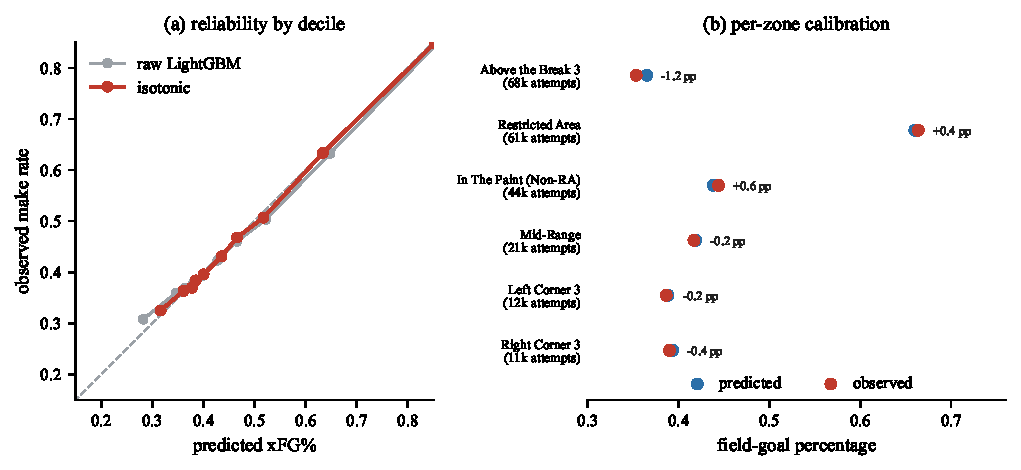
\includegraphics[width=\textwidth]{figures/fig1_xfg_reliability.pdf}
\caption{xFG on the 2024--25 holdout. (a) Reliability by predicted decile, raw
versus isotonic. (b) Per-zone predicted against
observed make rate, ordered by attempt volume, with the gap in percentage
points. The 511 backcourt attempts are omitted from panel (b); they sit far
below the plotted range.}
\label{fig:xfg}
\end{figure}

\subsection{xFTA fit, and why the fit statistic is the wrong one to read}

Out-of-fold Poisson deviance falls \SI{0.195}{\percent} against a season-mean
baseline. Per fold, from 2020--21 onward: 0.185, 0.168, 0.170, 0.254, 0.244 and
\SI{0.152}{\percent}. These are small numbers and we are not going to dress them
up. Whether a given possession yields a shooting foul is mostly unpredictable
from public context.

Table~\ref{tab:coef} gives the fitted coefficients. The two rate features carry
almost all the signal. The opponent term sits between 3.59 and 3.93 across folds
and the crew term between 1.71 and 2.53, both on a per-possession rate scale where
the league mean is about 0.18. Crews differ from each other in shooting-foul
frequency by enough to matter for an individual player's expected total, which is
consistent with the officiating literature
\citep{price2010racial, anderson2009officiating} and is the reason crew identity
is in the model at all.

The score-margin coefficient deserves a caution rather than a headline. It is the
smallest slope in the model and it moves by an order of magnitude across folds,
from \num{1.66e-5} in 2023--24 to \num{2.17e-4} in 2025--26, with no monotone
trend. We mention it because game state is known to influence foul calls, but the
estimate here is not stable enough to support an interpretation.

\begin{table}[t]
\centering
\small
\caption{Poisson GLM coefficients by held-out season. Each column is the fit on
the other five seasons.}
\label{tab:coef}
\begin{tabular}{lrrrrrr}
\toprule
& 2020--21 & 2021--22 & 2022--23 & 2023--24 & 2024--25 & 2025--26 \\
\midrule
Intercept                  & $-2.927$ & $-2.889$ & $-2.971$ & $-2.938$ & $-2.873$ & $-3.003$ \\
Period                     & $0.088$ & $0.086$ & $0.086$ & $0.081$ & $0.080$ & $0.086$ \\
Seconds remaining ($10^{-4}$) & $-1.36$ & $-1.53$ & $-1.46$ & $-1.44$ & $-1.40$ & $-1.53$ \\
Score margin ($10^{-4}$)   & $0.96$ & $0.95$ & $0.43$ & $0.17$ & $1.93$ & $2.17$ \\
Q4 or OT                   & $-0.096$ & $-0.088$ & $-0.090$ & $-0.088$ & $-0.082$ & $-0.088$ \\
Offence at home            & $0.015$ & $0.016$ & $0.016$ & $0.017$ & $0.018$ & $0.016$ \\
Opponent foul rate         & $3.844$ & $3.917$ & $3.881$ & $3.593$ & $3.929$ & $3.784$ \\
Crew foul rate             & $1.996$ & $1.751$ & $2.243$ & $2.404$ & $1.705$ & $2.527$ \\
\midrule
Anchor factor              & $1.025$ & $1.025$ & $1.016$ & $1.022$ & $1.021$ & $1.013$ \\
Deviance lift (\%)         & $0.185$ & $0.168$ & $0.170$ & $0.254$ & $0.244$ & $0.152$ \\
\bottomrule
\end{tabular}
\end{table}

\subsection{Reliability of the season-level metric}

The per-possession picture and the season-level picture disagree, and the
season-level one is what the metric is for.

Splitting each qualified player-season into odd and even games and correlating
FTAOE per 100 across halves gives $r = 0.841$ over \num{1691} player-seasons, a
Spearman-Brown full-season figure of $r = 0.914$
\citep{spearman1910correlation, brown1910some}. The implied padding constant is
$K = 67$ possessions, meaning a player's estimate should be shrunk toward the
league mean as though 67 league-average possessions were added to his
denominator. At the 300-possession qualifying threshold this implies a
reliability of 0.82; by 1000 possessions it is 0.94. Figure~\ref{fig:rel} shows
both.

Year-over-year correlation averages 0.85 across the five consecutive-season
pairs: 0.852 ($n = 208$), 0.834 ($n = 210$), 0.859 ($n = 219$), 0.865
($n = 222$) and 0.840 ($n = 217$). A metric that persists across seasons at 0.85
is measuring a property of the player rather than of the season.

\begin{figure}[t]
\centering
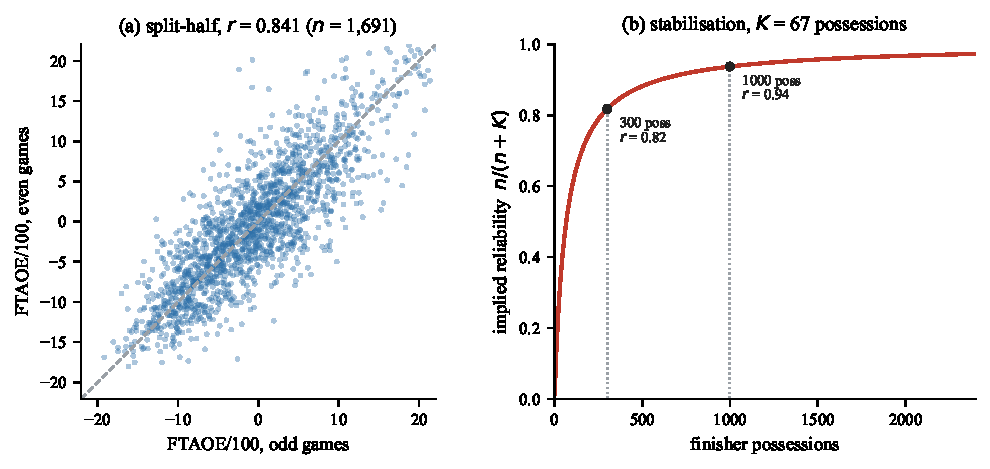
\includegraphics[width=\textwidth]{figures/fig2_ftaoe_reliability.pdf}
\caption{FTAOE reliability. (a) Odd-game against even-game FTAOE per 100 for
\num{1691} qualified player-seasons. (b) Implied reliability as a function of
possessions, $n/(n+K)$ with $K = 67$.}
\label{fig:rel}
\end{figure}

\subsection{Does withholding shooter identity cost anything?}
\label{sec:identity}

The model is context-only by construction. To test what that costs, we refitted
it twice on identical folds with identical anchoring, adding the finisher's
attributes. The \emph{archetype} arm adds height and position. The
\emph{identity} arm additionally adds the player's prior-season free-throw rate,
mean-imputed from training seasons only and paired with a missingness indicator.

Identity information does improve per-possession fit, substantially in relative
terms: mean fold lift rises from \SI{0.196}{\percent} to \SI{0.827}{\percent}
with height and position, and to \SI{1.786}{\percent} with prior-season rate
added. The ordering of players nonetheless survives. Rank correlation with the
context-only leaderboard is $\rho = 0.906$ for the archetype arm and
$\rho = 0.832$ for the identity arm (Figure~\ref{fig:identity}).

The tail moves more than the body, and we state this plainly because the
aggregate correlation would otherwise oversell the result. Overlap in the top ten
is 6 of 10 under the archetype arm and 2 of 10 under the identity arm. The
defensible claim is that the ordering is broadly preserved, not that the
leaderboard is unchanged.

What the identity arm actually demonstrates is circularity. Prior-season
free-throw rate is a measurement of the thing FTAOE is trying to measure, so
supplying it lets the model explain the signal away. Rudy Gobert's 2022--23
season moves from $+20.06$ to $-15.70$ FTAOE per 100, the largest change in the
sample, and he accounts for four of the eight largest drops. Told in advance that
Gobert draws fouls at a high rate, the model expects him to, and he stops
exceeding expectation. This is the argument for excluding identity features,
and it is an empirical one rather than a stylistic preference.

\begin{figure}[t]
\centering
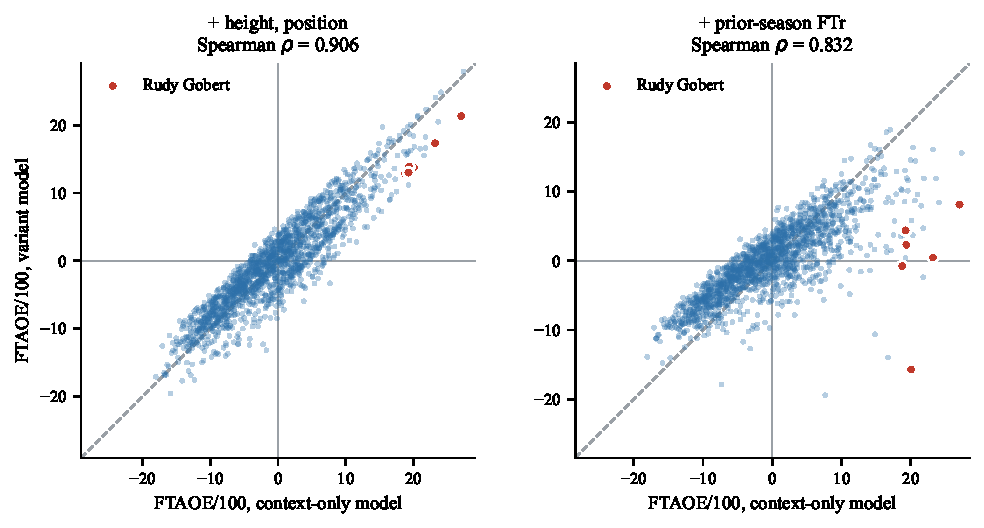
\includegraphics[width=\textwidth]{figures/fig3_identity_variant.pdf}
\caption{FTAOE per 100 under the context-only model against two identity-aware
variants, \num{1691} qualified player-seasons. Rudy Gobert's six seasons are
highlighted.}
\label{fig:identity}
\end{figure}

\subsection{Model family}

Two alternatives were fitted on the same folds with the same anchoring
(Table~\ref{tab:family}).

A multinomial logit over collapsed classes $\{0, 1, 2, 3^{+}\}$, with the top
class valued at its training-fold empirical mean of about 3.05, addresses the
lumpy support directly. It buys nothing. Deviance lift matches the Poisson GLM to
four decimal places and the resulting leaderboard is rank-identical
($\rho = 1.0000$, top-20 overlap 20 of 20).

A Poisson LightGBM on the same seven features, early stopped on a random
\SI{10}{\percent} of training rows so the evaluation fold is untouched, does
improve per-possession fit: \SI{0.254}{\percent} against \SI{0.196}{\percent}.
That improvement does not reach the season level. Full-season reliability moves
from 0.9135 to 0.9141, player-season calibration gets worse (slope 0.211 against
0.426), and the leaderboard is again nearly identical ($\rho = 0.9988$). The
extra flexibility captures per-possession structure that does not survive
aggregation, at a cost in calibration. We kept the GLM.

\begin{table}[t]
\centering
\small
\caption{Model family comparison. All arms share folds, anchoring and the
attributable-possession universe. Rank agreement is against the Poisson GLM.}
\label{tab:family}
\begin{tabular}{lccccc}
\toprule
& OOF lift (\%) & Split-half $r$ & Full-season $r$ & Calib.\ slope & Rank $\rho$ \\
\midrule
Poisson GLM        & 0.196 & 0.8408 & 0.9135 & 0.426 & --- \\
Multinomial        & 0.196 & 0.8408 & 0.9135 & 0.426 & 1.0000 \\
Poisson LightGBM   & \textbf{0.254} & 0.8419 & 0.9141 & 0.211 & 0.9988 \\
\bottomrule
\end{tabular}
\end{table}

\subsection{Calibration of the free-throw model}

Aggregate calibration holds, and is partly guaranteed: anchoring forces the mean
prediction to the season mean. Over player-seasons with at least 100 possessions,
mean predicted rate is 0.1835 against mean observed 0.1853, a gap of
\SI{0.95}{\percent}.

Calibration across the model's own predicted deciles is weak. Regressing observed
on predicted rate across deciles gives a slope of 0.426 with intercept 0.097, and
the highest predicted decile sits \SI{13.6}{\percent} below its prediction
(Figure~\ref{fig:calib}). We report this rather than the aggregate figure alone
because the aggregate figure on its own would be misleading.

The reason is structural. Predicted spread comes from context and covers only
0.174 to 0.197, while observed spread across player-seasons is dominated by the
player skill the model is deliberately blind to. Sorting player-seasons by
predicted rate therefore does not sort them by observed rate, and the narrow
predictor range attenuates the fitted slope further. A context-only model
\emph{should} fail this test; a model that passed it would be encoding the
residual it is supposed to leave behind. What the metric requires is that the
expectation be unbiased in aggregate, which it is.

\begin{figure}[t]
\centering
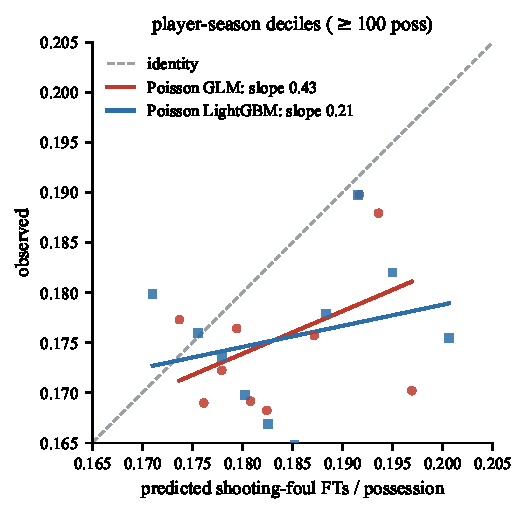
\includegraphics[width=0.52\textwidth]{figures/fig4_calibration.pdf}
\caption{Player-season decile calibration for the Poisson GLM and the boosted
alternative. Neither tracks the identity line, and the boosted model tracks it
less closely.}
\label{fig:calib}
\end{figure}

\subsection{Benchmarks}

League aggregates reconstructed from our pipeline match published values across
all six seasons: restricted area 0.641--0.671, paint outside the restricted area
0.427--0.446, mid-range 0.406--0.420, corner three 0.383--0.397, above-the-break
three 0.346--0.360, league effective field-goal percentage 0.531--0.546, and
league free-throw percentage 0.775--0.784.

\section{Findings}

The 2024--25 leaders in total FTAOE are Giannis Antetokounmpo ($+311.8$), James
Harden ($+192.5$), Jimmy Butler III ($+190.7$) and Shai Gilgeous-Alexander
($+175.0$). The bottom is Mikal Bridges ($-120.0$), Klay Thompson ($-104.5$),
Payton Pritchard ($-103.7$) and Buddy Hield ($-97.3$). The ordering is
unsurprising, which is the point: a metric that ranked unfamiliar names at the
top would be measuring noise or a bug, and this one recovers the players whose
foul-drawing is widely recognised without ever being told who they are.

The two lenses separate players that a single number would merge. Averaged across
seasons, Stephen Curry is $+5.4$ percentage points on shot-making with FTAOE of
$-23$: an outstanding shot-maker who draws fewer shooting fouls than his shot
diet predicts. Giannis Antetokounmpo, Joel Embiid, Zion Williamson and
Gilgeous-Alexander are all strongly positive on FTAOE. The correlation structure
here is what makes the residual worth computing separately rather than folding
into a single efficiency number.

On officiating, the crew rate coefficient is positive and sizeable in every fold
(1.71 to 2.53). Crews differ in how often shooting fouls are called, by enough to
shift an individual player's expected free-throw total over a season. We stop
there. The model identifies variation associated with assigned crews; it does not
establish that any crew is biased with respect to any player or team, and the
design cannot support that claim because crew assignment is not random with
respect to teams, venues or scheduling.

\section{Limitations}
\label{sec:limitations}

\paragraph{Shot selection is inside the residual, not the baseline.}
Because the model conditions on context rather than on the finisher, a player who
is skilled at manufacturing contact-prone situations is credited for it in FTAOE
rather than having it absorbed into his expectation. FTAOE therefore measures
foul-drawing given the possessions a player actually finished, which mixes
contact craft with the decision to seek contact. Disentangling them needs a
model of shot selection \citep{sandholtz2020measuring}, which we have not built.

\paragraph{No tracking data.}
Defender distance, contest level, shot clock, touch time and dribble count are
unavailable per shot from public sources. This caps xFG discrimination near
AUC 0.66, well below tracking-era models \citep{cervone2016multiresolution}, and
removes the most plausible physical mediator of foul drawing from the FTAOE
model.

\paragraph{Bonus state is unobserved.}
The public feed carries no bonus indicator, so \texttt{q4\_or\_ot} stands in for
it. Penalty free throws are excluded from the target, which limits the damage,
but late-period foul dynamics are only crudely represented.

\paragraph{Per-decile calibration is weak.}
As reported above, the slope is 0.426. We have argued this is expected for a
context-only model, but a reader who wants a model whose predicted player-season
rates track observed rates should not use this one for that purpose.

\paragraph{Known coverage gaps.}
About \num{1800} shots per season in 2021--22 through 2024--25, roughly
\SI{0.8}{\percent}, appear in play-by-play without a matching
\texttt{shotchartdetail} row and so carry no location. They are excluded from
xFG. Action type describes the attempt rather than the outcome, but its
granularity may correlate weakly with outcome; this is standard practice in
public expected-field-goal models and we accept and disclose it. A 2025--26
change in how end-of-period heaves are charged creates a cross-season
discontinuity in long-range attempts, with roughly 50 attempts beyond 40 feet at
a \SI{44}{\percent} make rate against roughly 600 at 2--4\% in earlier seasons.

\paragraph{One held-out season for the xFG benchmark.}
The xFG metrics in Table~\ref{tab:xfg}, including the leakage comparison, come
from a single holdout season, 2024--25. The FTAOE results use all six seasons
out-of-fold. We do not claim the xFG numbers generalise beyond that season.

\section{Practitioner implications and future work}
\label{sec:practice}

The usable output is a per-player, per-season rate with a known reliability curve.
Because $K = 67$ possessions, a player crosses $r = 0.5$ after about 67
possessions and $r = 0.9$ after about 600. That is a small enough sample to be
useful in-season, and it means FTAOE stabilises considerably faster than most
box-score-derived rate statistics. A team evaluating a target with two months of
data can use it; a team using it to separate two players 20 possessions apart
cannot.

Three practical uses follow. Player evaluation gains a component that raw
free-throw attempts actively distorts, since the raw count rewards role. Because
the metric is anchored per season, cross-season comparison is meaningful even
across rule-enforcement changes, which matters for any multi-year projection.
And because the model carries an explicit crew term, a team can quantify how much
of a player's free-throw variance across a season is attributable to officiating
assignment rather than to his own play.

The obvious extension is a shot-selection model that would move the
contact-seeking component out of the residual and let FTAOE isolate contact craft
proper. Beyond that, the same construction transfers to any league with public
play-by-play and foul attribution, and we have applied the pipeline to eight
non-NBA competitions, though the reliability analysis in this paper is NBA-only.
What will not transfer without tracking data is a sharper expected field-goal
model, and that remains the binding constraint on the shot-value side of the
system.

\section*{Reproducibility}

All model artifacts, the validation scripts and the figure-generating code are in
the repository named on the title page. The variant comparisons in
Sections~\ref{sec:identity} and following are produced by
\texttt{variant\_archetype.py} and \texttt{variant\_model\_family.py}, each of
which asserts that its baseline arm reproduces the shipped model before its
variant arms are read. The bibliography was generated programmatically from
records resolved against CrossRef and OpenAlex.

\bibliography{references}

\end{document}
